\begin{figure}[H]
    \centering
    \begin{subfigure}{0.95\linewidth}
        \centering
        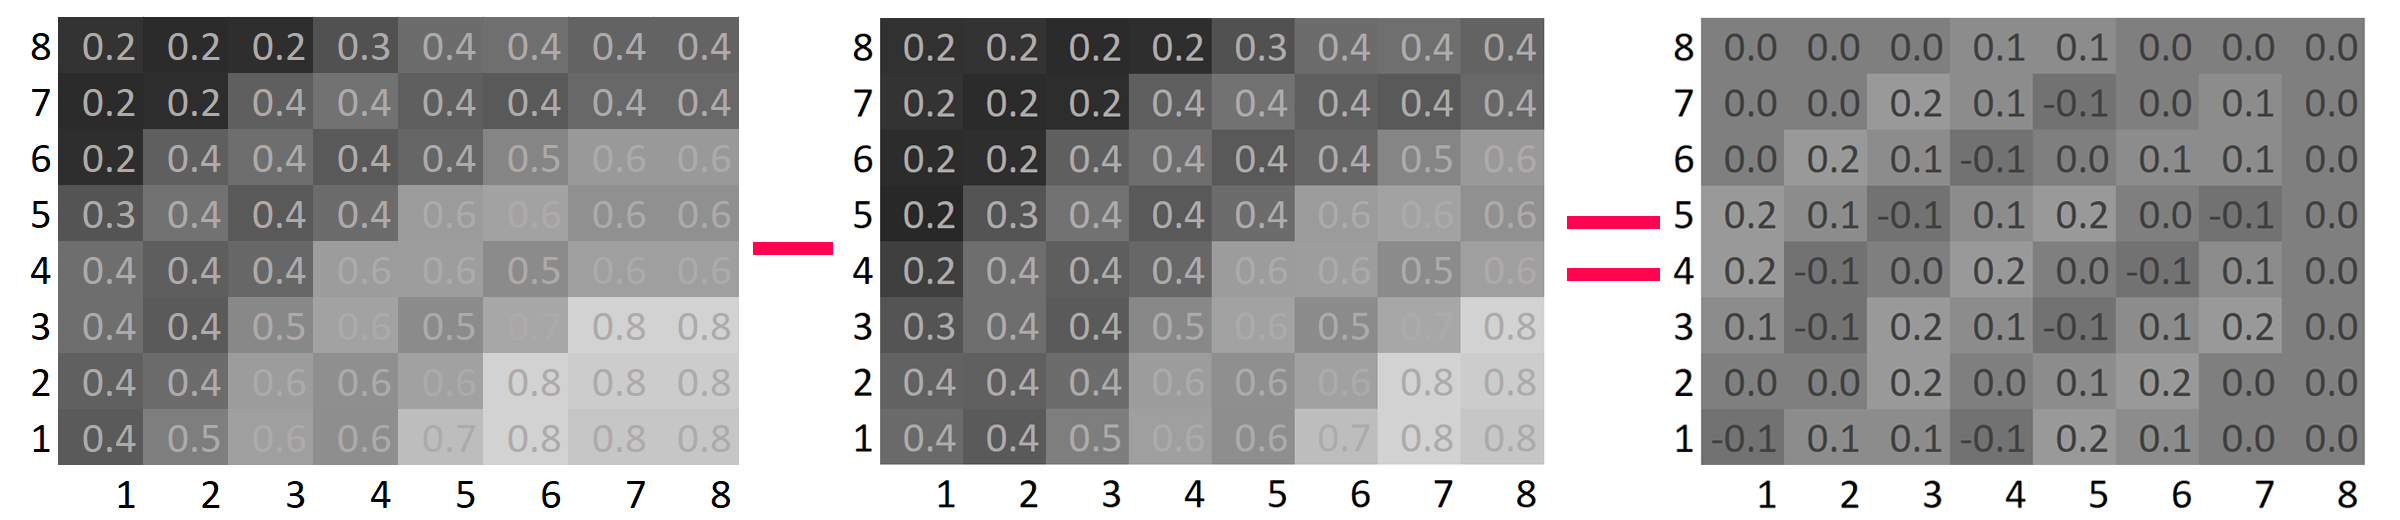
\includegraphics[width=0.9\linewidth]{image/finite_difference/x_derivertive.png}
    \end{subfigure}
    \caption{ตัวอย่างการหาอนุพันธ์บนภาพเฉดเทา}
    \label{figure:x-derivertive}
\end{figure}